\documentclass[a4paper,12pt]{article}

% Paquetes básicos
\usepackage[utf8]{inputenc}
\usepackage[T1]{fontenc}
\usepackage[spanish]{babel}
\usepackage{graphicx}
\usepackage{xcolor}
\usepackage{lipsum}
\usepackage{geometry}
\geometry{top=3cm, bottom=3cm, left=2.5cm, right=2.5cm}

% Paquetes para diseño
\usepackage{titlesec}
\usepackage{fancyhdr}
\usepackage{amsmath}
\usepackage{amssymb}
\usepackage{hyperref}

% Paquetes para el entorno lstlisting
\usepackage{listings}
\usepackage{inconsolata}

% Paquete para fondo
\usepackage{background}
\usepackage{pdfpages}

% Configuración de lstlisting
\lstset{
    language=Ruby,
    basicstyle=\ttfamily\small,
    keywordstyle=\color{blue}\bfseries,
    stringstyle=\color{teal},
    commentstyle=\color{gray}\itshape,
    numbers=left,
    numberstyle=\tiny\color{gray},
    backgroundcolor=\color{black!5},
    frame=single,
    rulecolor=\color{black!50},
    breaklines=true,
    captionpos=b,
    showstringspaces=false,
    extendedchars=true,
}

% Configuración de título
\titleformat{\section}{\normalfont\Large\bfseries}{\thesection}{1em}{}

% Información del documento
\title{
    \vspace{-2cm}
    
\includegraphics[width=0.3\textwidth]{images/etsiit.png} \\ % Cambia el logo si es necesario
    \LARGE Ingeniería Informática + ADE\\
    \large Universidad de Granada (UGR)\\[1cm]
}
\author{\textbf{Autor:} Ismael Sallami Moreno}
\date{\textbf{Asignatura:} Programación y Diseño Orientado a Objetos (PDOO)}

% Configuración del fondo
\backgroundsetup{
    scale=1,
    color=black,
    opacity=0.2,
    angle=0,
    position=current page.south,
    vshift=0pt,
    hshift=0pt,
    contents={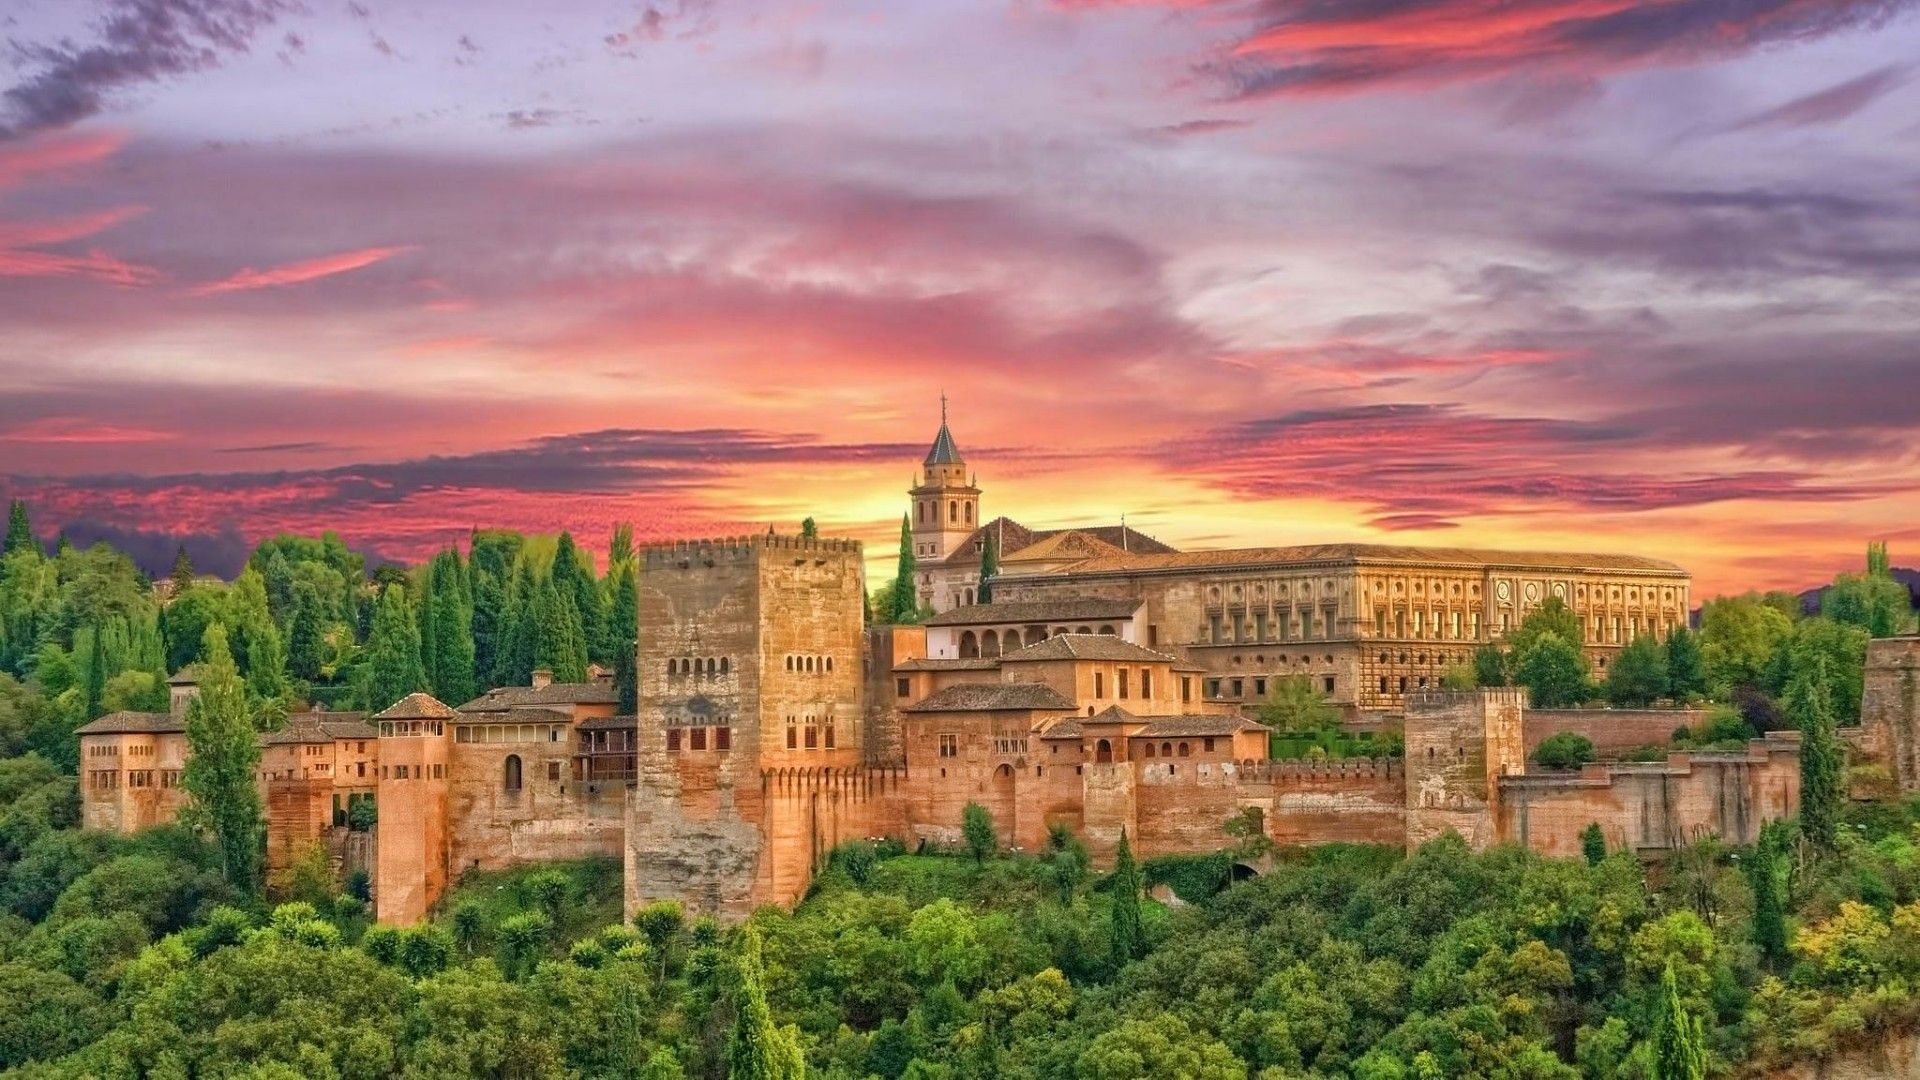
\includegraphics[width=\paperwidth,height=\paperheight,keepaspectratio]{images/granada.jpg}}
}

% Inicio del documento
\begin{document}

% Portada
\maketitle
\thispagestyle{empty}

\begin{center}
    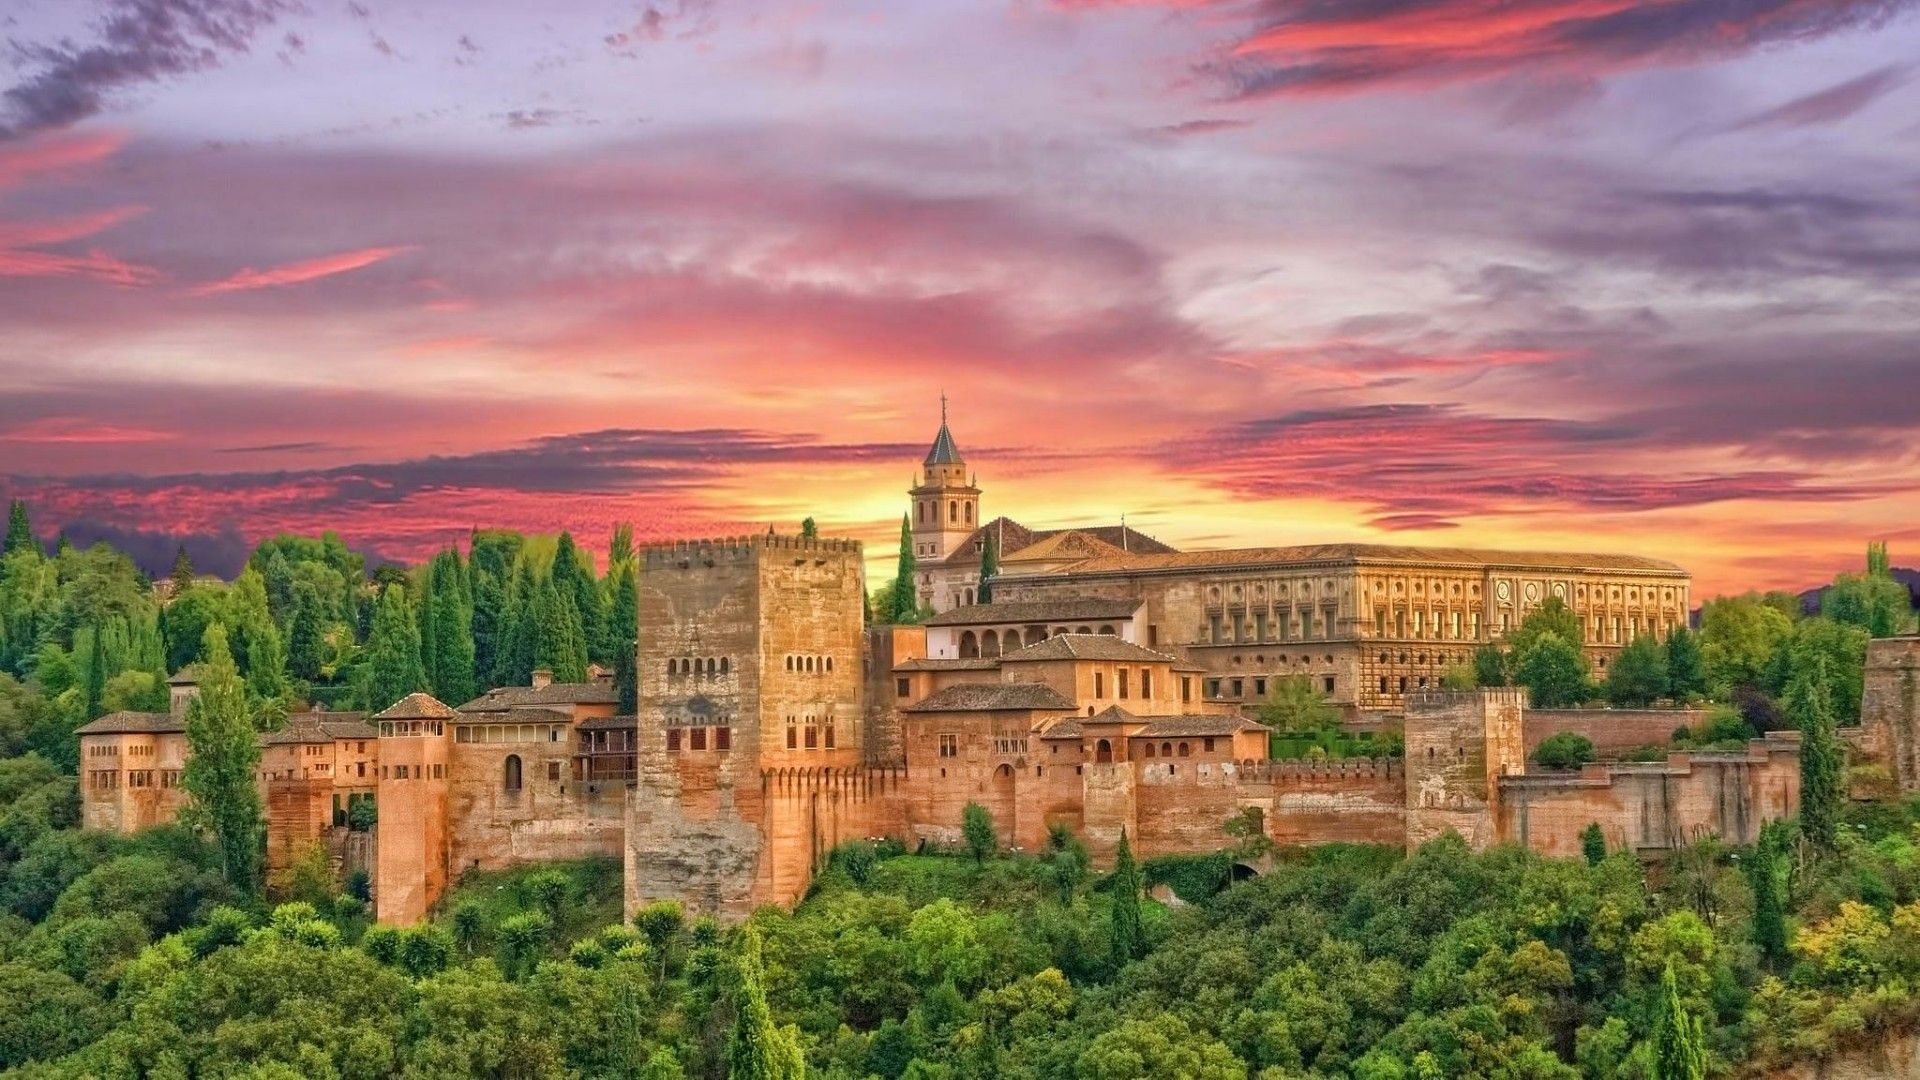
\includegraphics[width=\textwidth,height=0.4\textheight,keepaspectratio]{images/granada.jpg} \\ % Añade tu imagen de fondo
    \vfill
\end{center}

\newpage

% Índice (opcional)
\tableofcontents
\newpage

\section{Teoría}
\subsection{Tema 1}
\subsubsection{Conceptos Básicos}
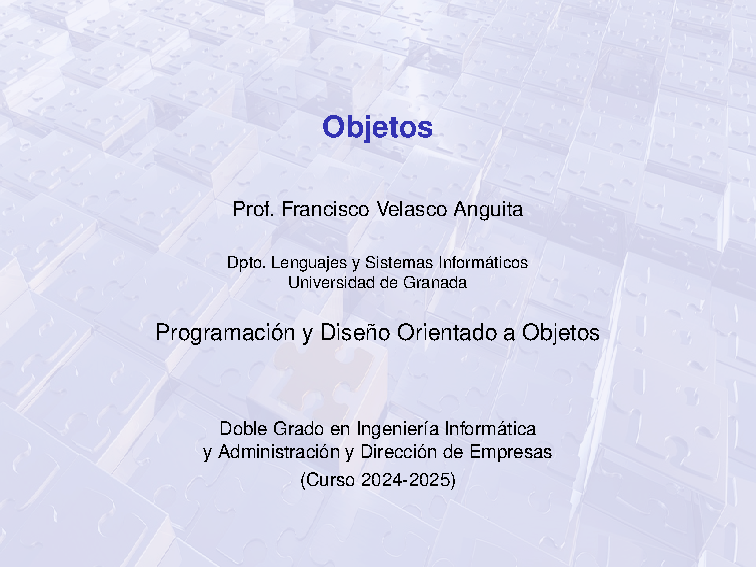
\includepdf[pages=-]{../Diapositivas/t1/t1.pdf}
%incluir un archivo rb con input:
\href{https://github.com/ElblogdeIsmael/ElblogdeIsmael.github.io/tree/main/Asignaturas/Tercer%20A%C3%B1o/PDOO/Teoria/Diapositivas/}{Ejemplo en ruby de buen y mal diseño}

\subsection{Tema 2}
\subsubsection{Atributos y Métodos}
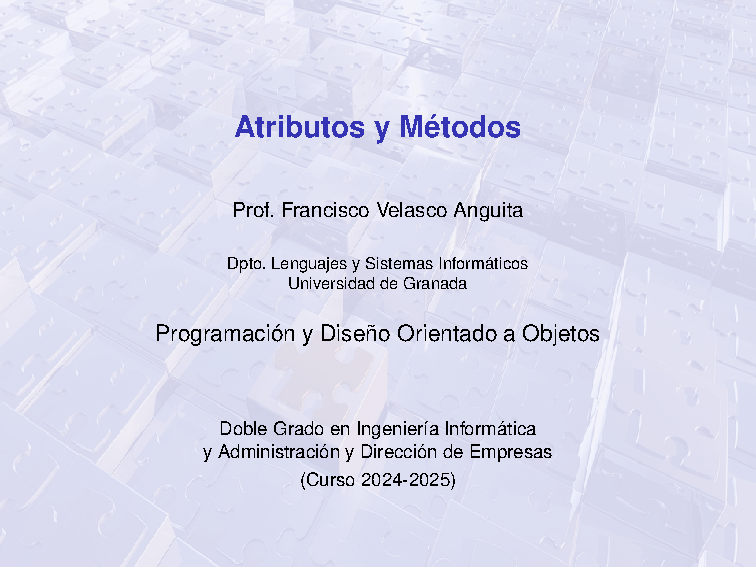
\includepdf[pages=-]{../Diapositivas/t2/a.pdf}
\subsubsection{Construcción de Objetos}
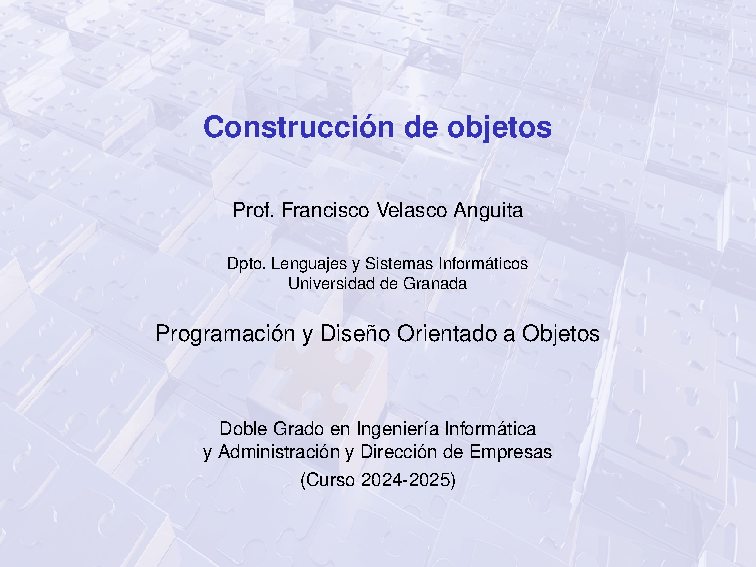
\includepdf[pages=-]{../Diapositivas/t2/b.pdf}
\subsubsection{Consultores y Modificadores}
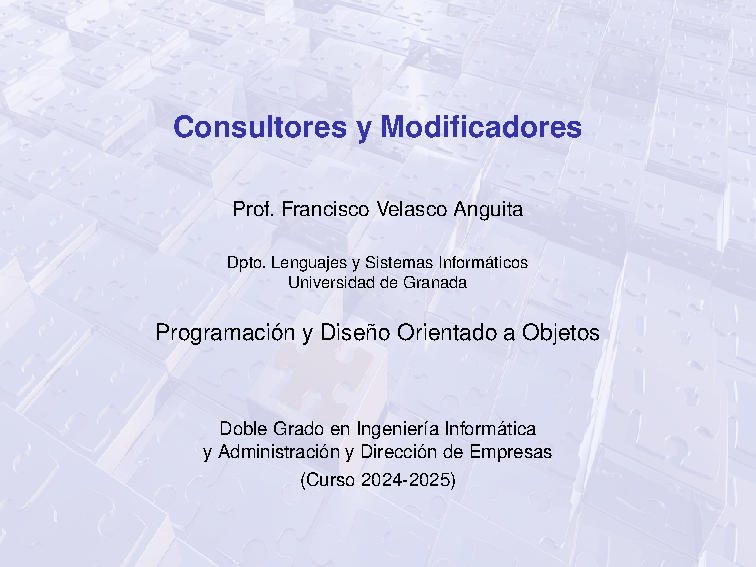
\includepdf[pages=-]{../Diapositivas/t2/c.pdf}
\subsubsection{Elementos de Agrupación}
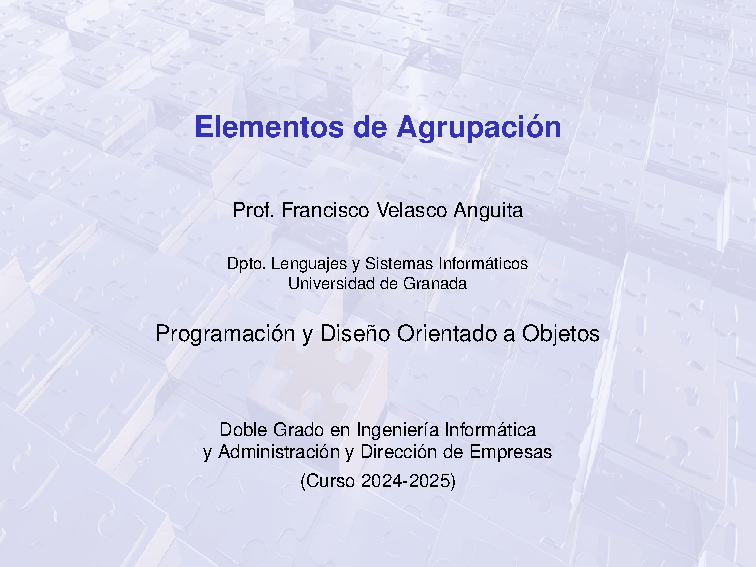
\includepdf[pages=-]{../Diapositivas/t2/d.pdf}
\subsubsection{Diagramas Estructurales}
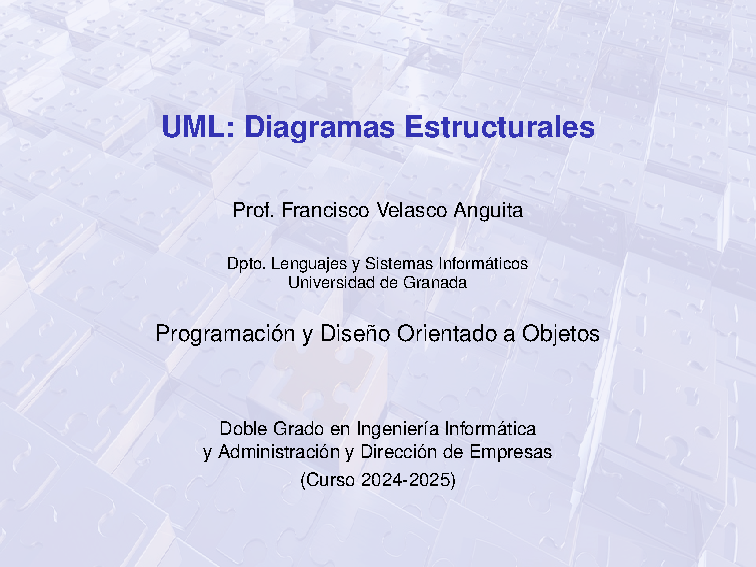
\includepdf[pages=-]{../Diapositivas/t2/e.pdf}
\subsubsection{Diagramas de Interacción}
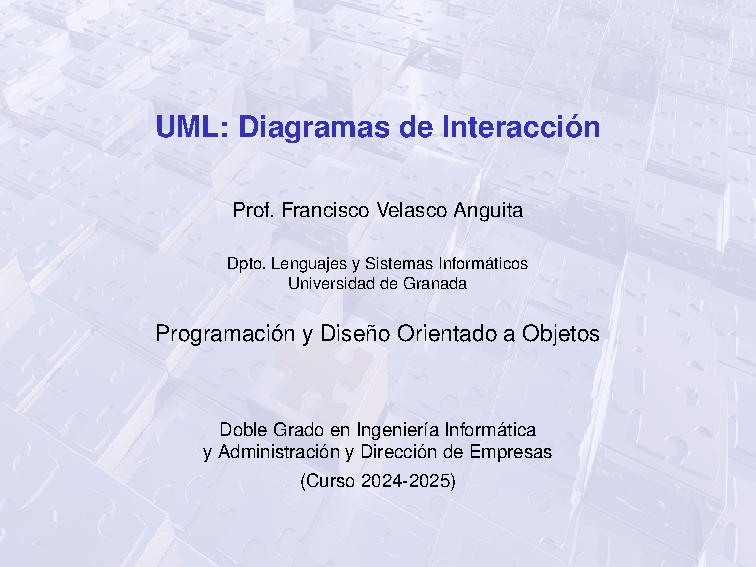
\includepdf[pages=-]{../Diapositivas/t2/f.pdf}

\subsection{Tema 3}
\subsubsection{Herencia}
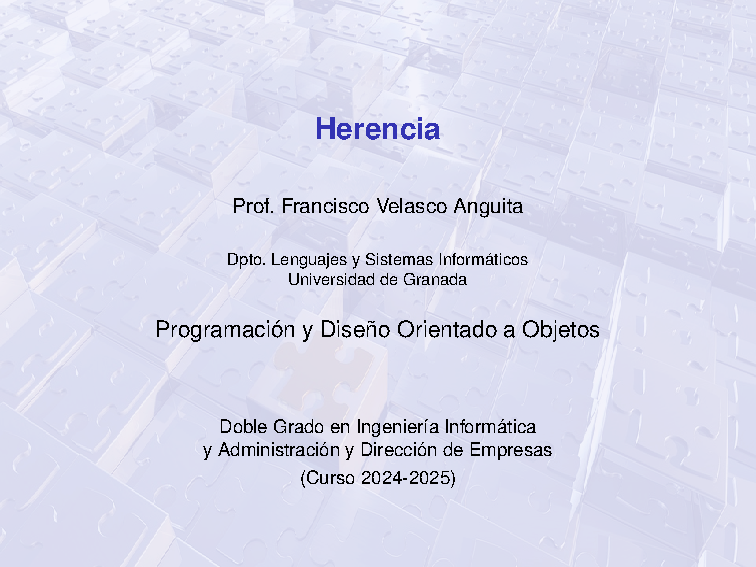
\includepdf[pages=-]{../Diapositivas/t3/Herencia.pdf}
\subsubsection{Visibilidad}
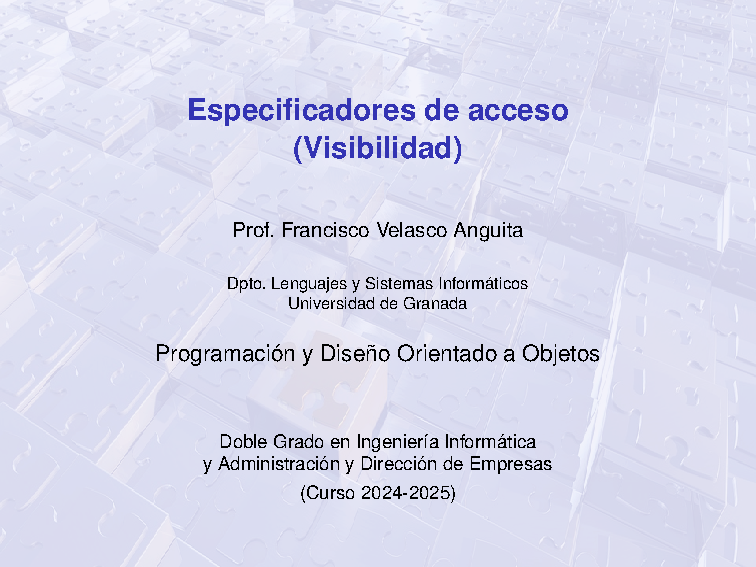
\includepdf[pages=-]{../Diapositivas/t3/Visibilidad.pdf}
\subsubsection{Polimorfismo}
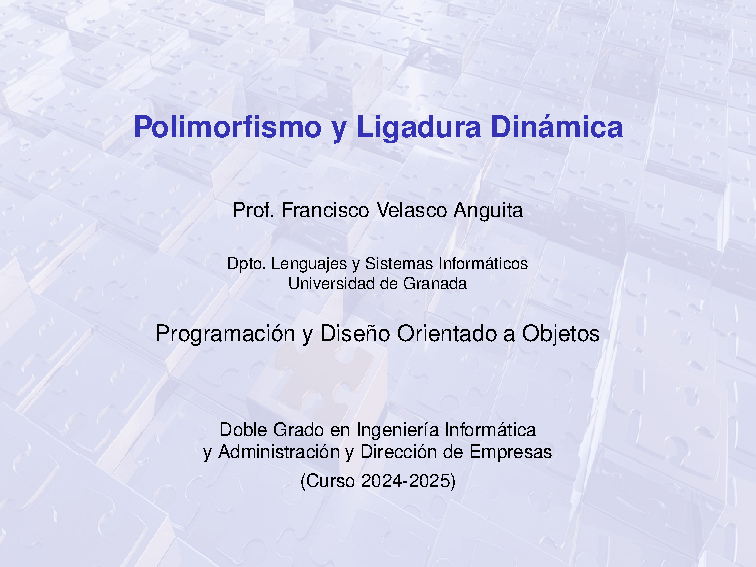
\includepdf[pages=-]{../Diapositivas/t3/Polimorfismo.pdf}
\subsubsection{Clases Abstractas}
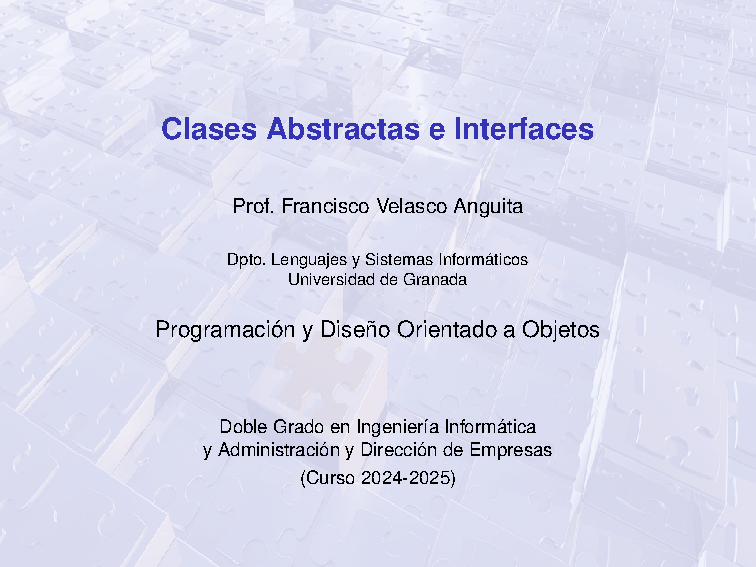
\includepdf[pages=-]{../Diapositivas/t3/clasesAbstractas.pdf}
\subsubsection{Clases Parametrizables}
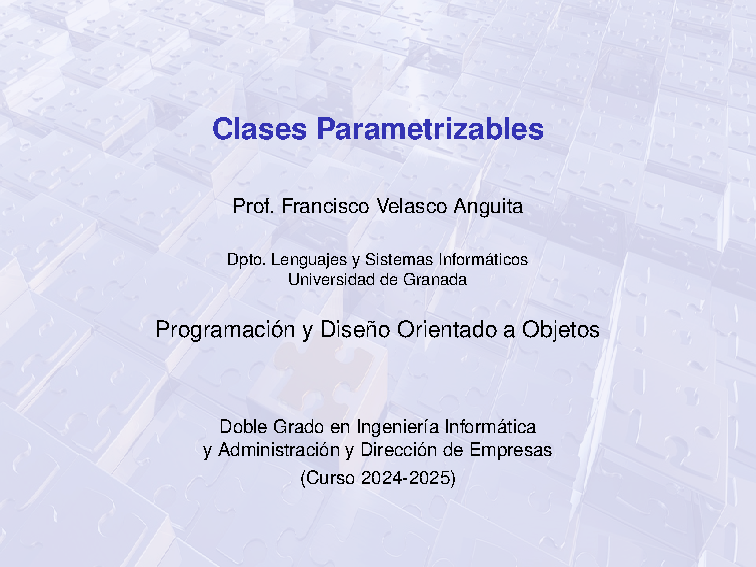
\includepdf[pages=-]{../Diapositivas/t3/clasesParametrizables.pdf}
\subsubsection{Herencia en Ámbito de Clases}
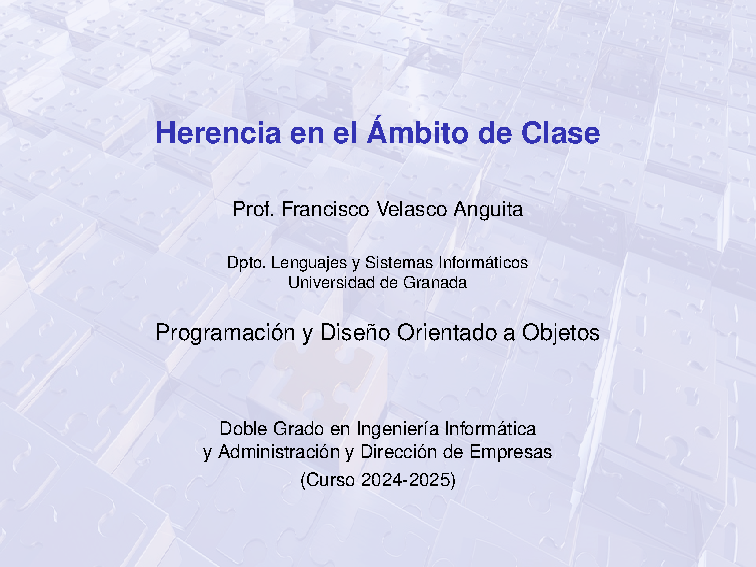
\includepdf[pages=-]{../Diapositivas/t3/HerenciaAmbitoClase.pdf}
\subsubsection{Herencia Múltiple}
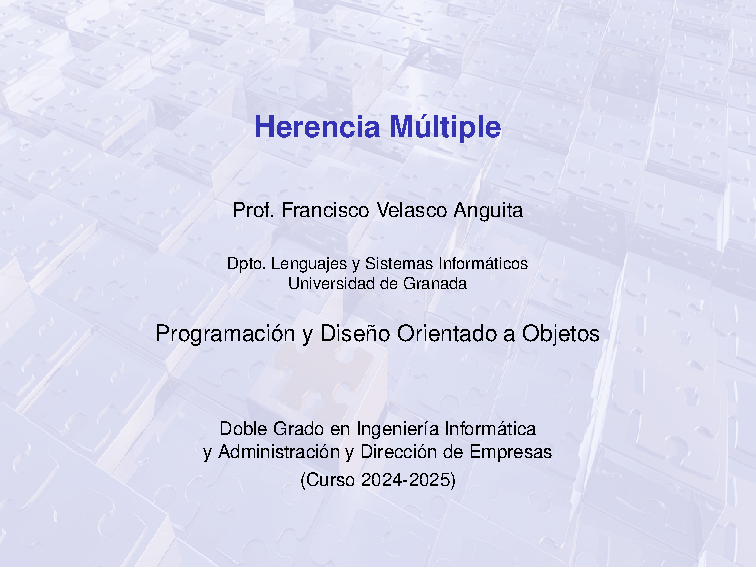
\includepdf[pages=-]{../Diapositivas/t3/HerenciaMultiple.pdf}

\subsection{Tema 4}
\subsubsection{Modelo Vista Controlador}
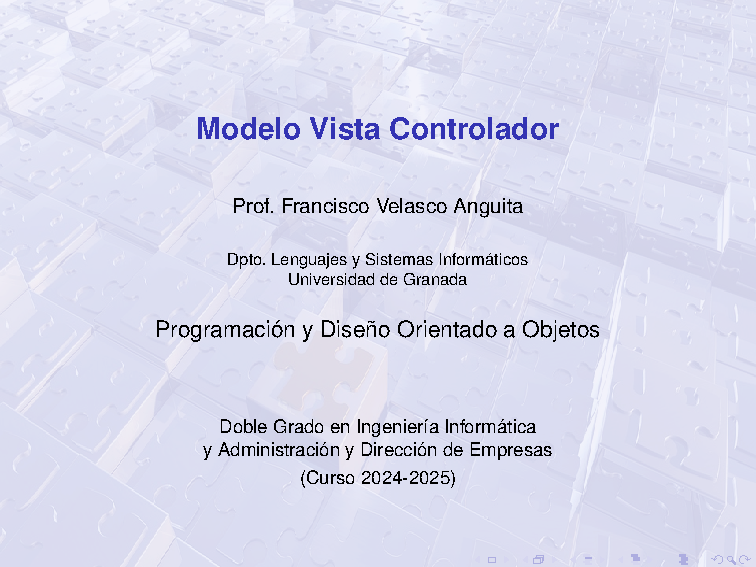
\includepdf[pages=-]{../Diapositivas/t4/MVC.pdf}
\subsubsection{Reflexión}
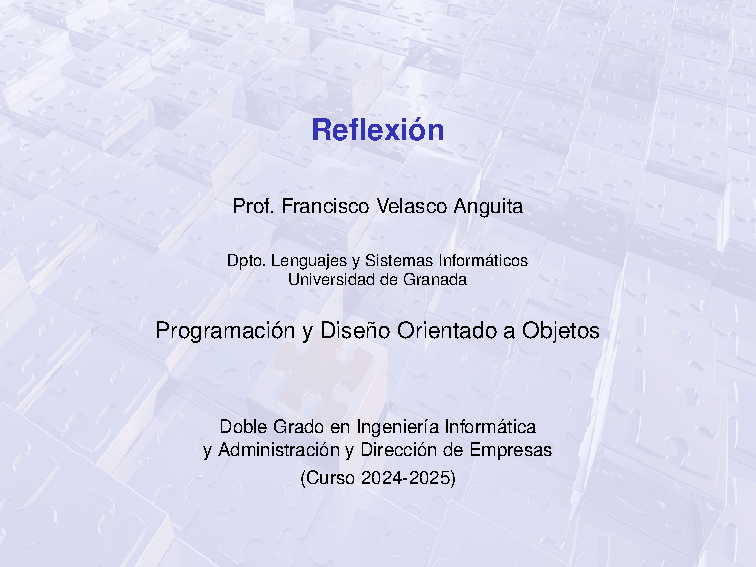
\includepdf[pages=-]{../Diapositivas/t4/Reflexion.pdf}
\subsubsection{Copia de Objetos}
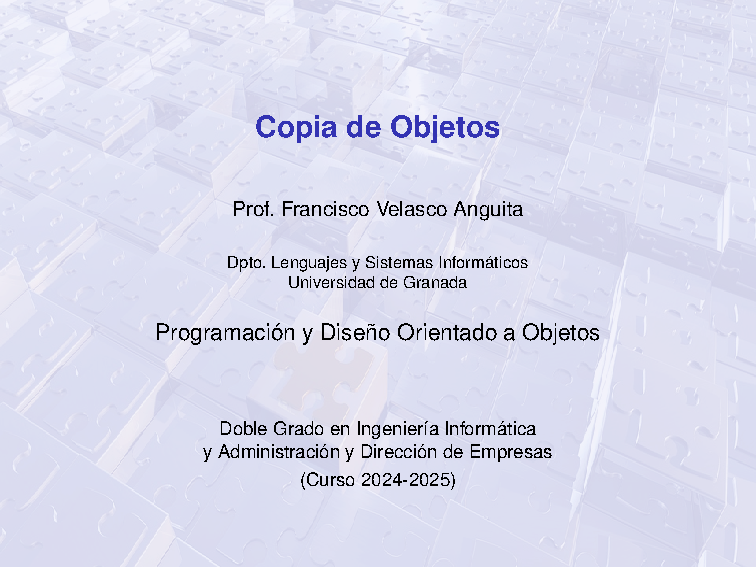
\includepdf[pages=-]{../Diapositivas/t4/CopiaObjetos.pdf}


\section{Relaciones de Problemas}
\subsection{Relación 1 con soluciones}
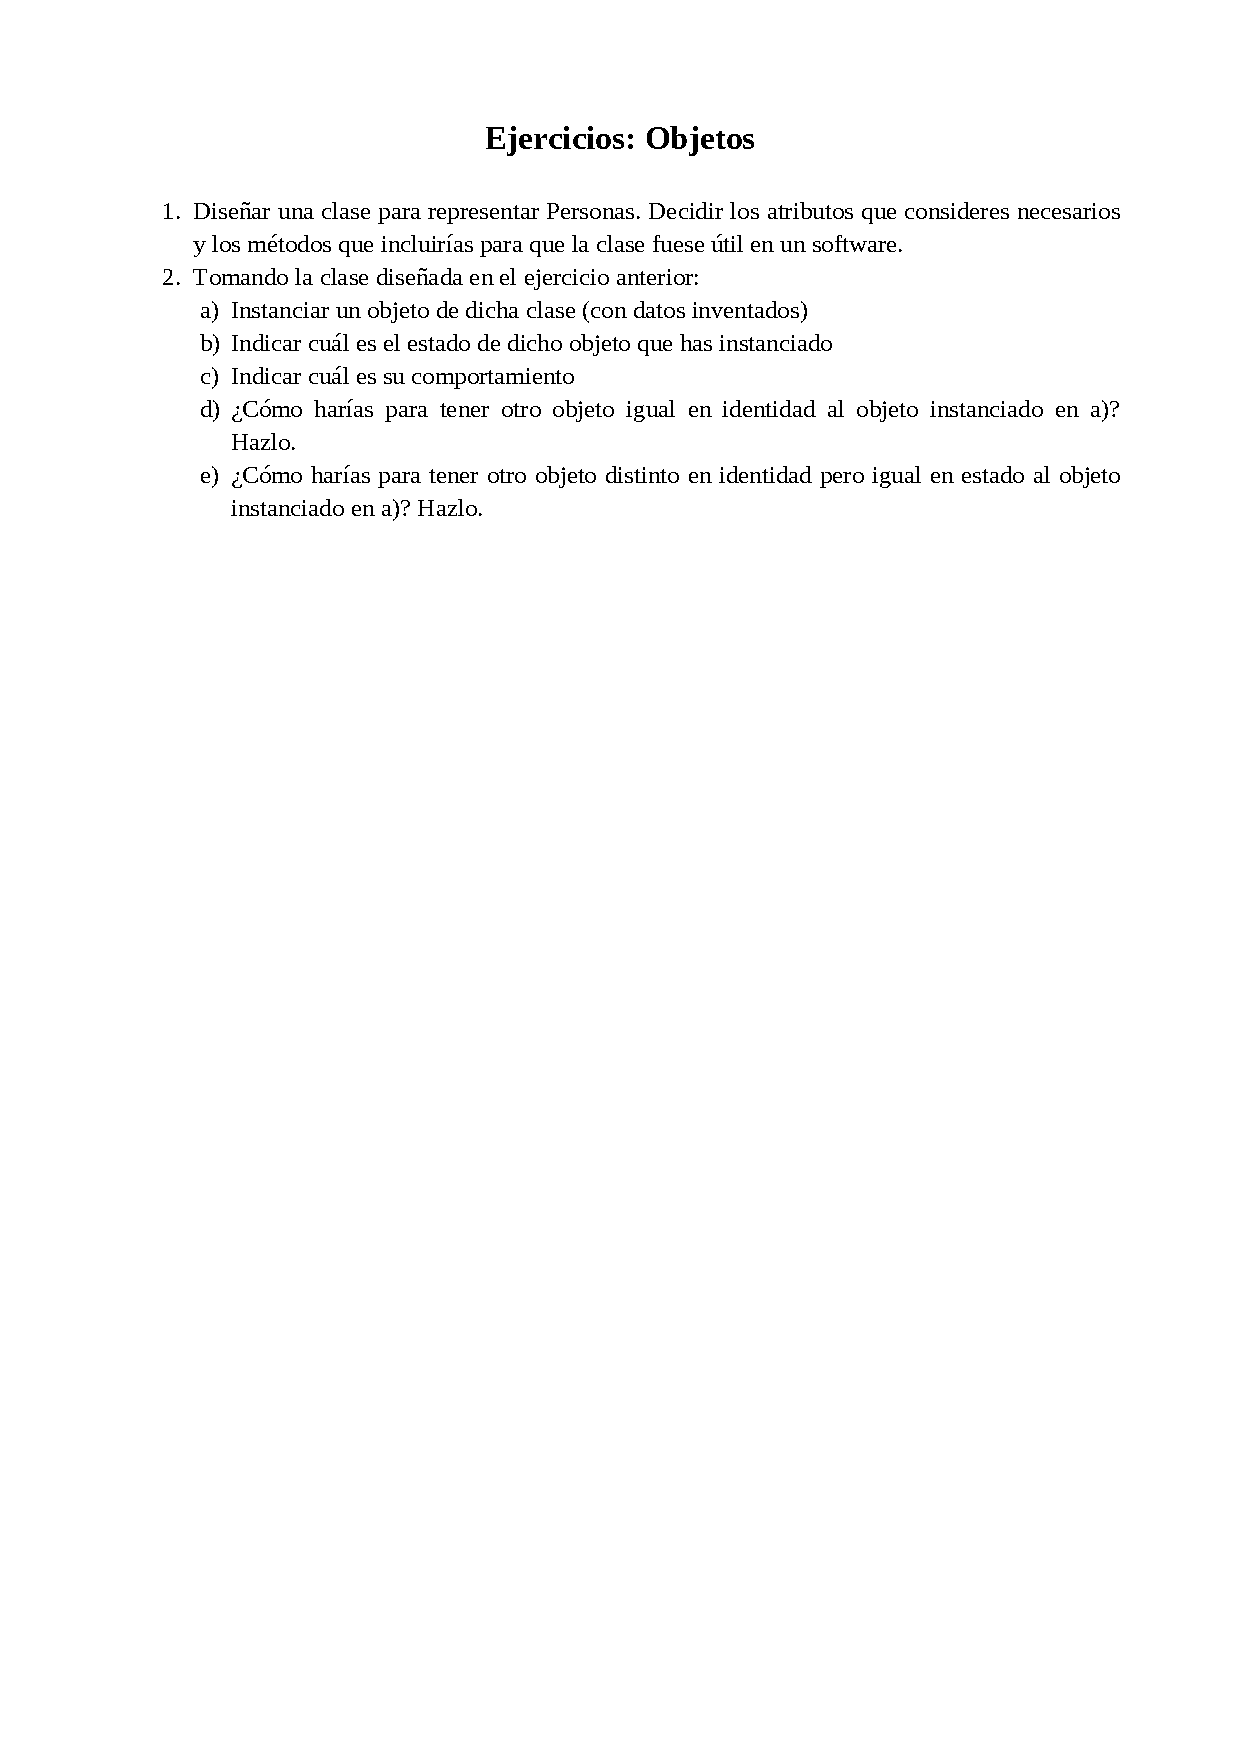
\includepdf[pages=-]{../RelacionesEjercicios/t1.pdf}

\subsection{Relación 2 con soluciones}
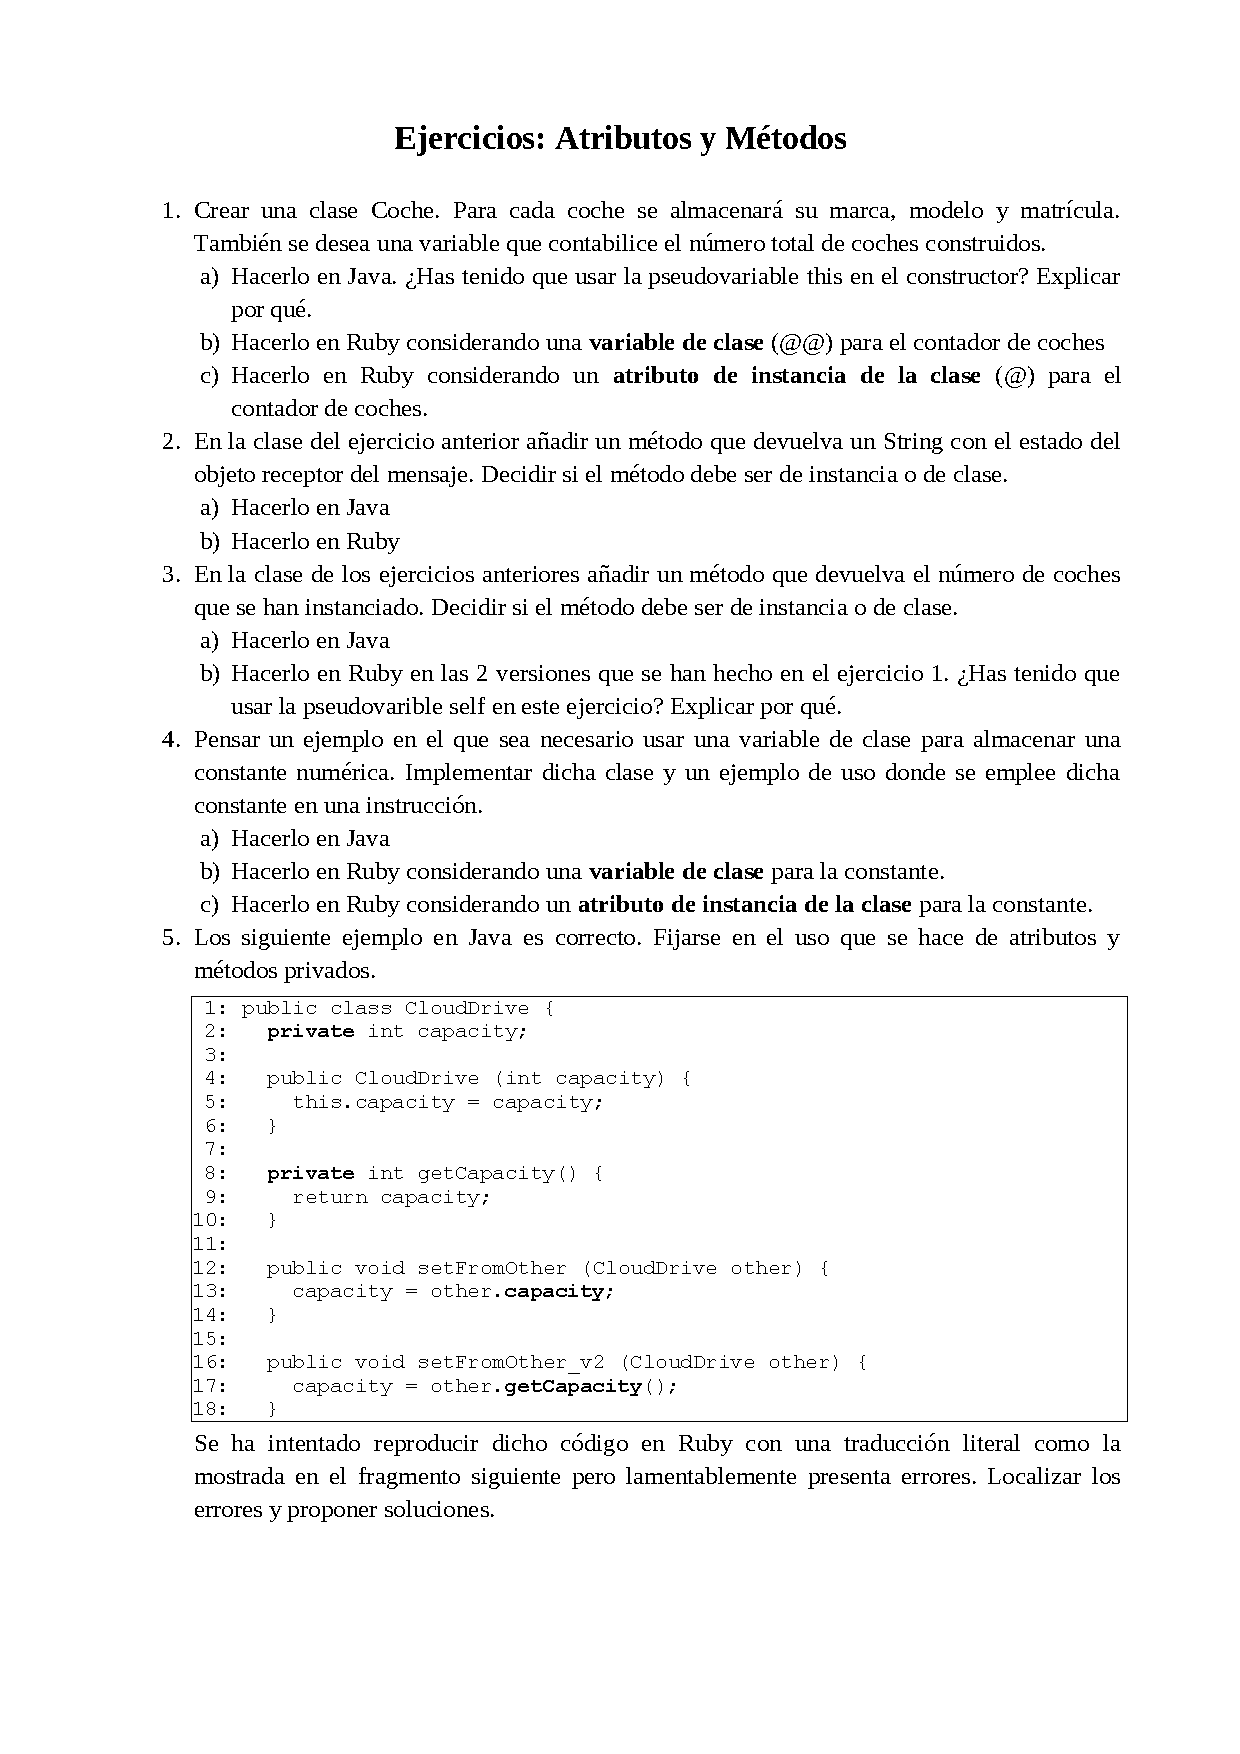
\includepdf[pages=-]{../RelacionesEjercicios/t2.pdf}

\subsection{Relación 3}
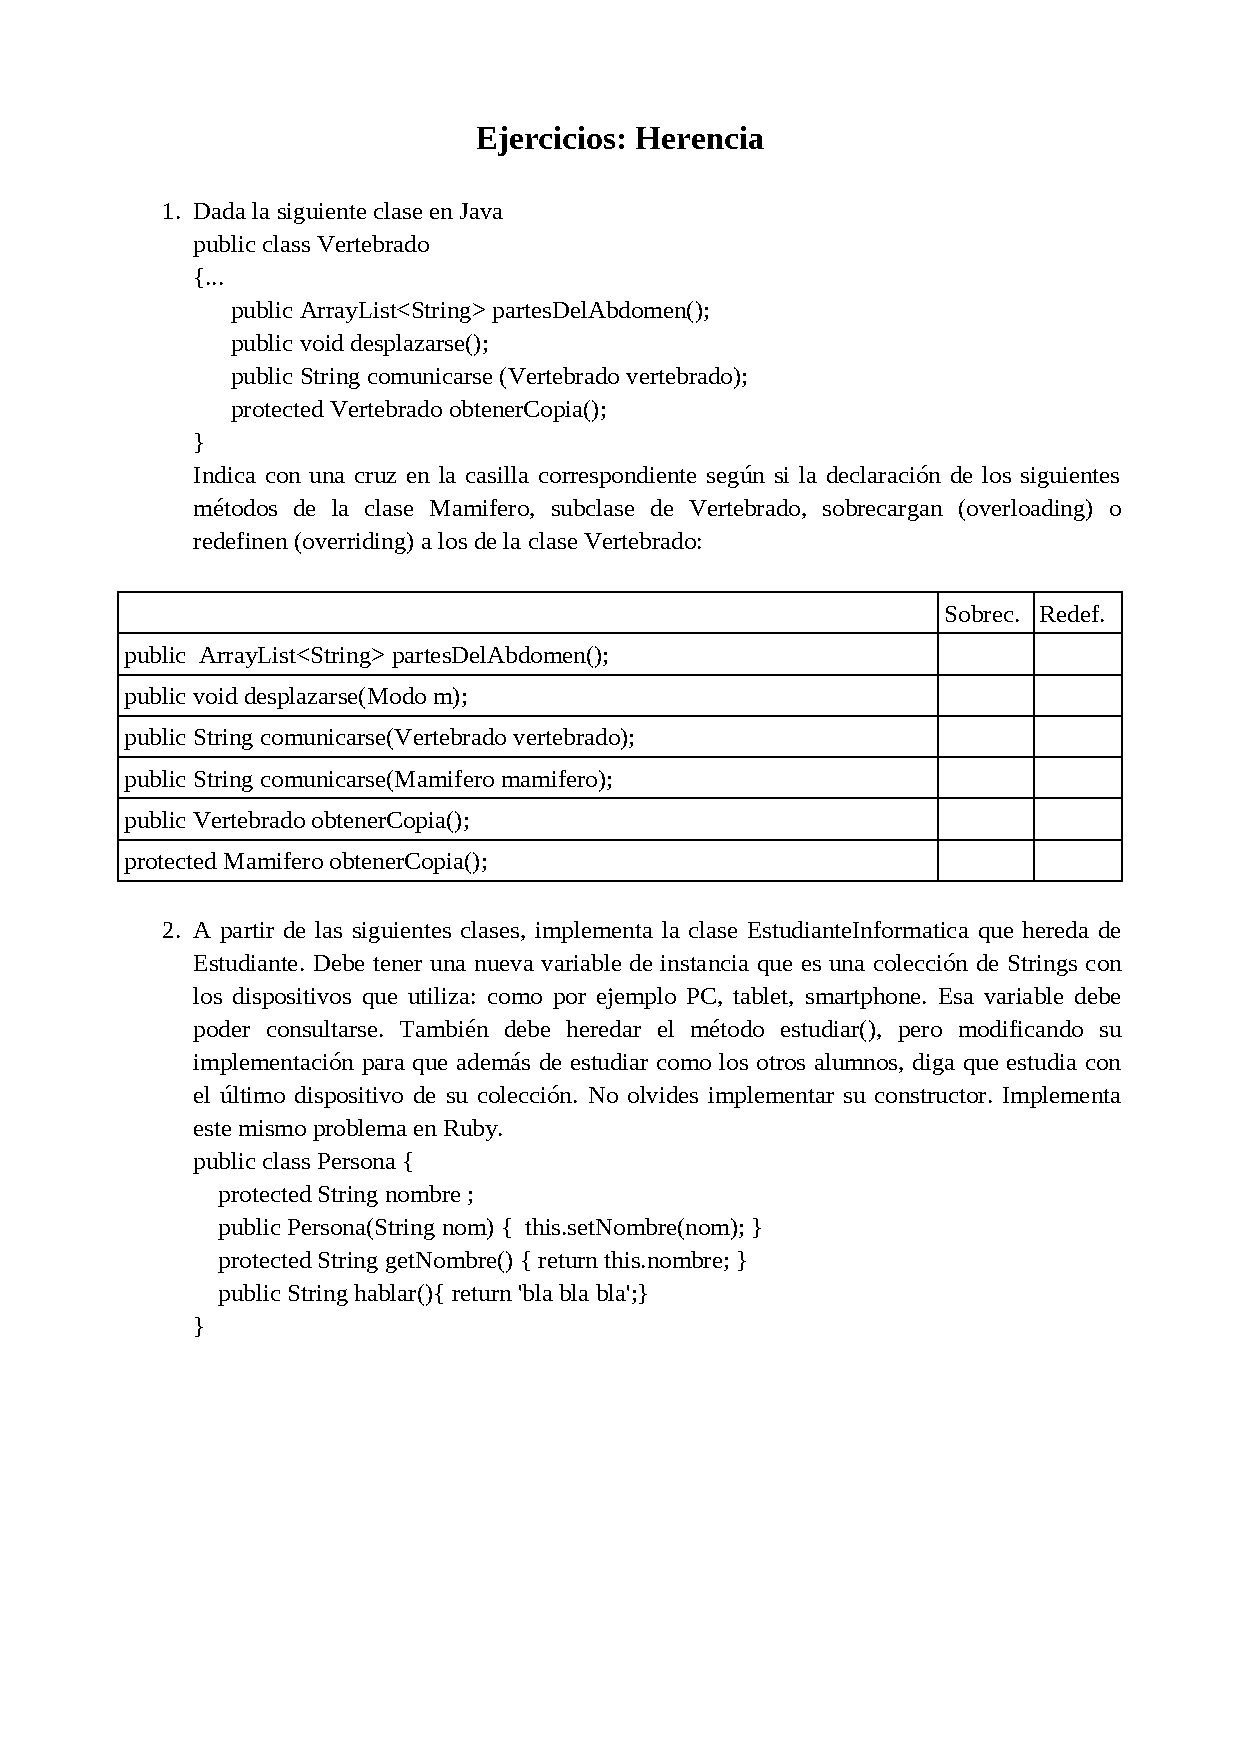
\includepdf[pages=-]{../RelacionesEjercicios/t3.pdf}
\subsubsection{Soluciones}
\includepdf[pages=2-]{../RelacionesEjercicios/Solt3/ETSIIT/build/solt3.pdf}
\section{Exámenes}
\subsection{Examen 1}
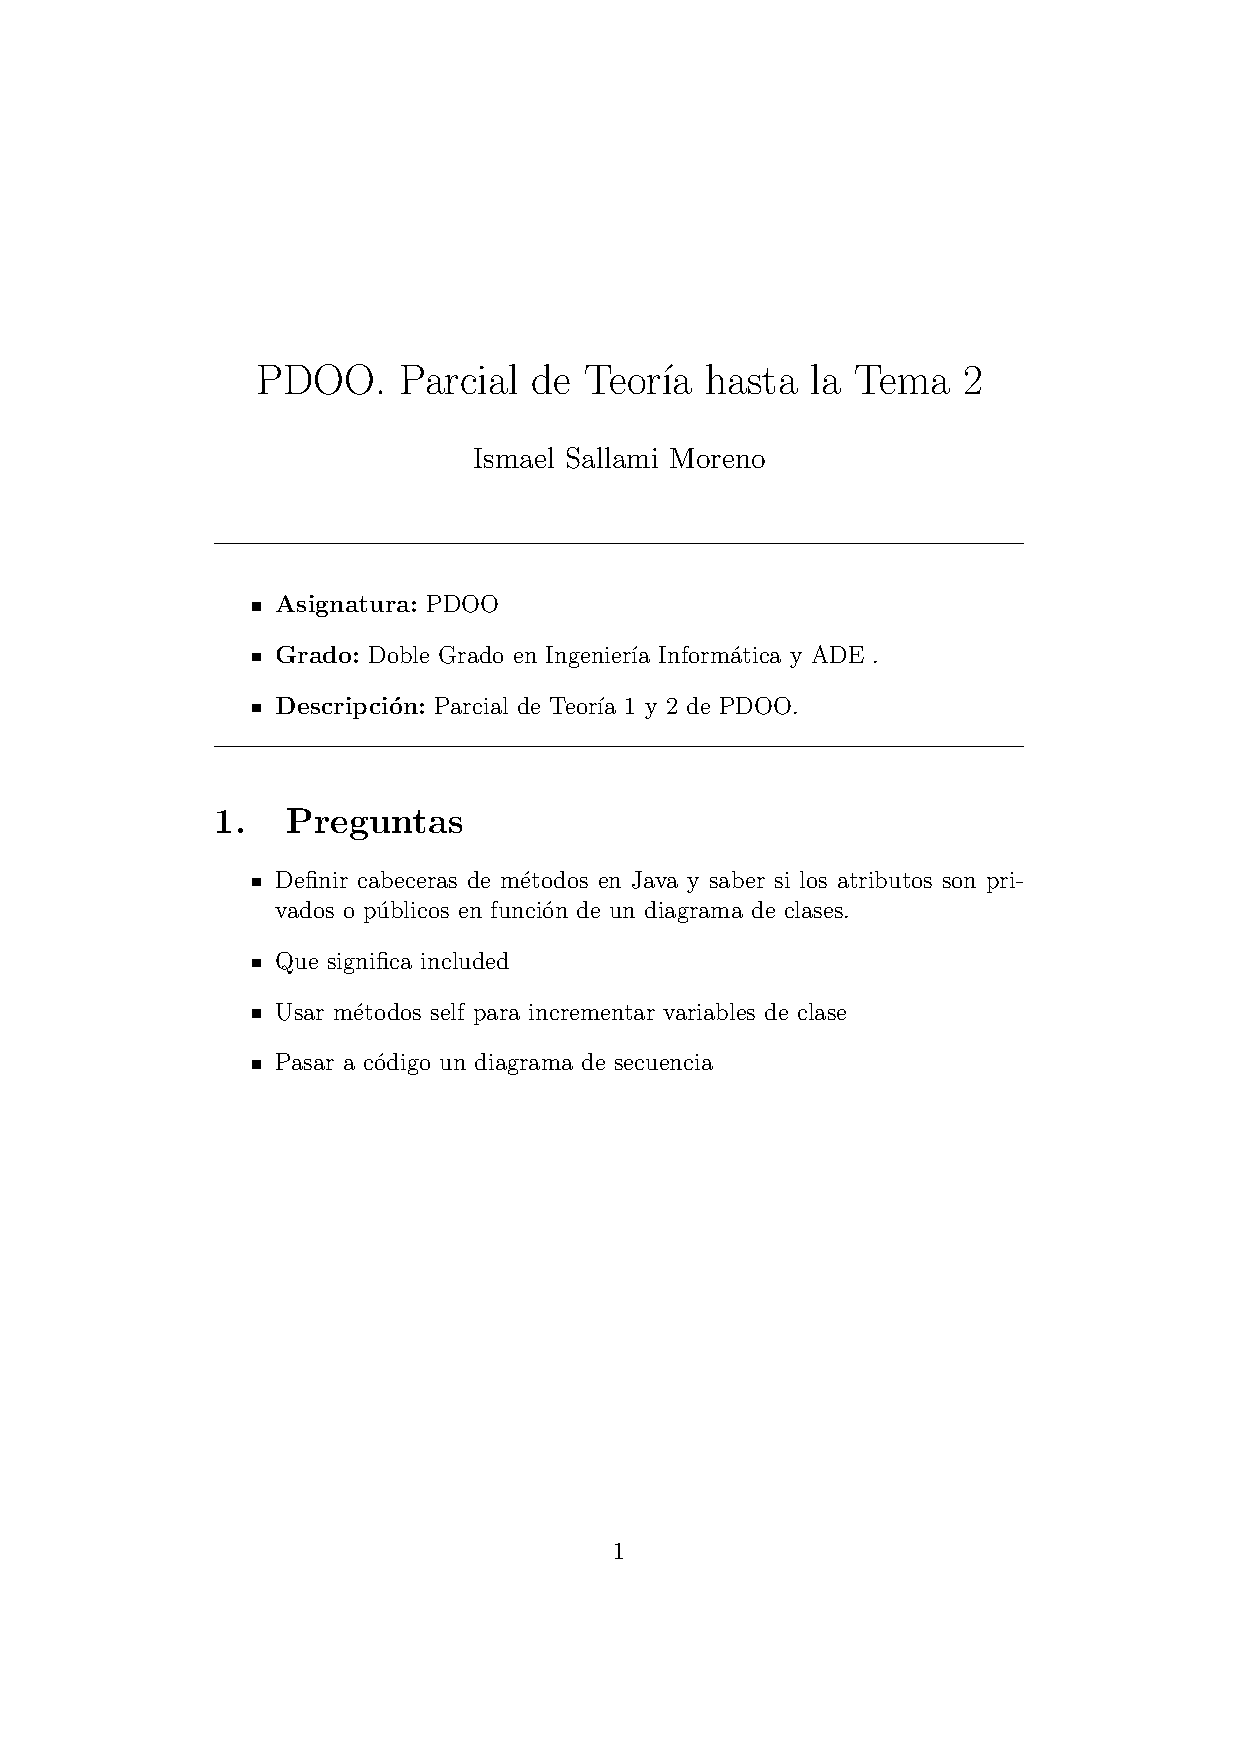
\includepdf[pages=-]{../../Examenes/parcial1Teoria.pdf}

\end{document}
